% !TEX root = ../main.tex

\chapter{实验与结果}

\section{数据集介绍}

本章我们基于两个中文数据集进行实验,测试本文所提出的NER方案的性能。
数据集分别是使用Weibo NER数据集\parencite{peng-dredze-2016-improving}和MSRA数据集\parencite{levow-2006-third}。

\subsection{Weibo NER数据集}
Weibo NER数据集是面向社交媒体的中文命名实体识别数据集。该数据集包括训练集(1350个句子)、验证集(269个句子)、测试集(270个句子),
实体类型包括地缘政治实体(GPE.NAM)、地名(LOC.NAM)、机构名(ORG.NAM)、人名(PER.NAM)及其对应的代指(以NOM为结尾)。
表~\ref{tab:weibo_ner}是它的统计信息

\begin{table}[!hpt]
    \caption[Weibo NER数据集统计信息]{Weibo NER数据集统计信息}
    \label{tab:weibo_ner}
    \centering
    \begin{tabular}{lrrr} \toprule
     &  句子数 & 字符数 & 实体数 \\ \midrule
    训练集 & 1350 & 73728 & 1885 \\
    测试集 & 270 & 14810 & 414 \\
    验证集 & 269 & 14463 & 389 \\ \bottomrule
    \end{tabular}
\end{table}

其中各类实体的具体数量如表~\ref{tab:weibo_ner_entity_class}

\begin{table}[!hpt]
    \caption[Weibo NER数据集各类实体统计信息]{Weibo NER数据集各类实体统计信息}
    \label{tab:weibo_ner_entity_class}
    \centering
    \begin{tabular}{lrrr} \toprule
    实体类型 & 训练集 & 测试集 & 验证集 \\ \midrule
    地缘政治实体(GPE.NAM \& GPE.NOM) & 213 & 49 & 27 \\
    地名(LOC.NAM \& LOC.NOM) & 107 & 28 & 12 \\
    机构名(ORG.NAM \& ORG.NOM) & 225 & 56 & 52 \\
    人名(PER.NAM \& PER.NOM) & 1340 & 281 & 298 \\ \bottomrule
    \end{tabular}
\end{table}


\subsection{MSRA数据集}
MSRA数据集是面向新闻领域的中文命名实体识别数据集。
该数据集包括训练集(46364个句子)、测试集(4365个句子),实体类型包括地名(LOC)、人名(NAME)、组织名(ORG)。
表~\ref{tab:MSRA_ner}是它的统计信息

\begin{table}[!hpt]
    \caption[MSRA数据集统计信息]{MSRA数据集统计信息}
    \label{tab:MSRA_ner}
    \centering
    \begin{tabular}{lrrr} \toprule
     &  句子数 & 字符数 & 实体数 \\ \midrule
    训练集 & 46364 & 2169879 & 74703 \\
    验证集 & 4365 & 172601 & 6181 \\ \bottomrule
    \end{tabular}
\end{table}

其中各类实体的具体数量如表~\ref{tab:MSRA_ner_entity_class}

\begin{table}[!hpt]
    \caption[MSRA数据集各类实体统计信息]{MSRA数据集各类实体统计信息}
    \label{tab:MSRA_ner_entity_class}
    \centering
    \begin{tabular}{lrr} \toprule
    实体类型 & 训练集 & 验证集 \\ \midrule
    地名(LOC) & 36517 & 2877 \\
    机构名(ORG) & 20571 & 1331 \\
    人名(PER) & 17615 & 1973 \\ \bottomrule
    \end{tabular}
\end{table}

\section{评价指标}

在本实验中,我们对各类实体以及所有实体预测的准确率(Precision,P)、召回率(Recall,R)和F1值(F1 score,F)进行评估。
对于一个两类预测问题,给定一个实例,其预测结果只有两种可能,正例和负例。则真实标签与
预测标签的组合总共会出现四种情况:

\begin{itemize}
    \item \textbf{真正例(True Positive, TP)}:真实情况为正例,预测结果也为正例
    \item \textbf{假正例(False Positive, FP)}:真实情况为负例,预测结果为正例
    \item \textbf{假负例(False Negative, FN)}:真实情况为正例,预测结果为负例
    \item \textbf{真正例(True Negative, TN)}:真实情况为负例,预测结果也为负例
\end{itemize}

Precision、Recall与F1 score的计算方式如下:

\begin{equation}
    P = \frac{TP}{TP + FP}
\end{equation}

\begin{equation}
    R = \frac{TP}{TP + FN}
\end{equation}

\begin{equation}
    F = \frac{2 \times P \times R}{P + R}
\end{equation}

\section{实验配置}

本实验的环境为Pytorch深度学习环境,表~\ref{tab:hyper_parameter_setting}列出了实验的超参数细节

\begin{table}[!hpt]
    \caption[实验超参数对照表]{实验超参数对照表}
    \label{tab:hyper_parameter_setting}
    \centering
    \begin{tabular}{lc} \toprule
        参数 & 值 \\ \midrule
        嵌入维度(Embedding\_num) & 128 \\
        隐藏层维度(Hidden\_num) & 64 \\
        学习率(Learning Rate) & 0.01 \\
        优化算法  & torch.optim.Adam \\
        Weibo数据集(epoch, batch\_size) & [(200, 200), (200, 100), (200, 50), (500, 100)] \\
        MSRA数据集(epoch, batch\_size) & [(1000, 1000), (200, 1000), (200, 500), (200, 200)] \\ \bottomrule
    \end{tabular}
\end{table}


\section{实验结果}

\subsection{BiLSTM-GRU}

\subsubsection{Weibo数据集结果}

\begin{figure}[!htp]
    \centering
    \label{fig:weibo_result}
    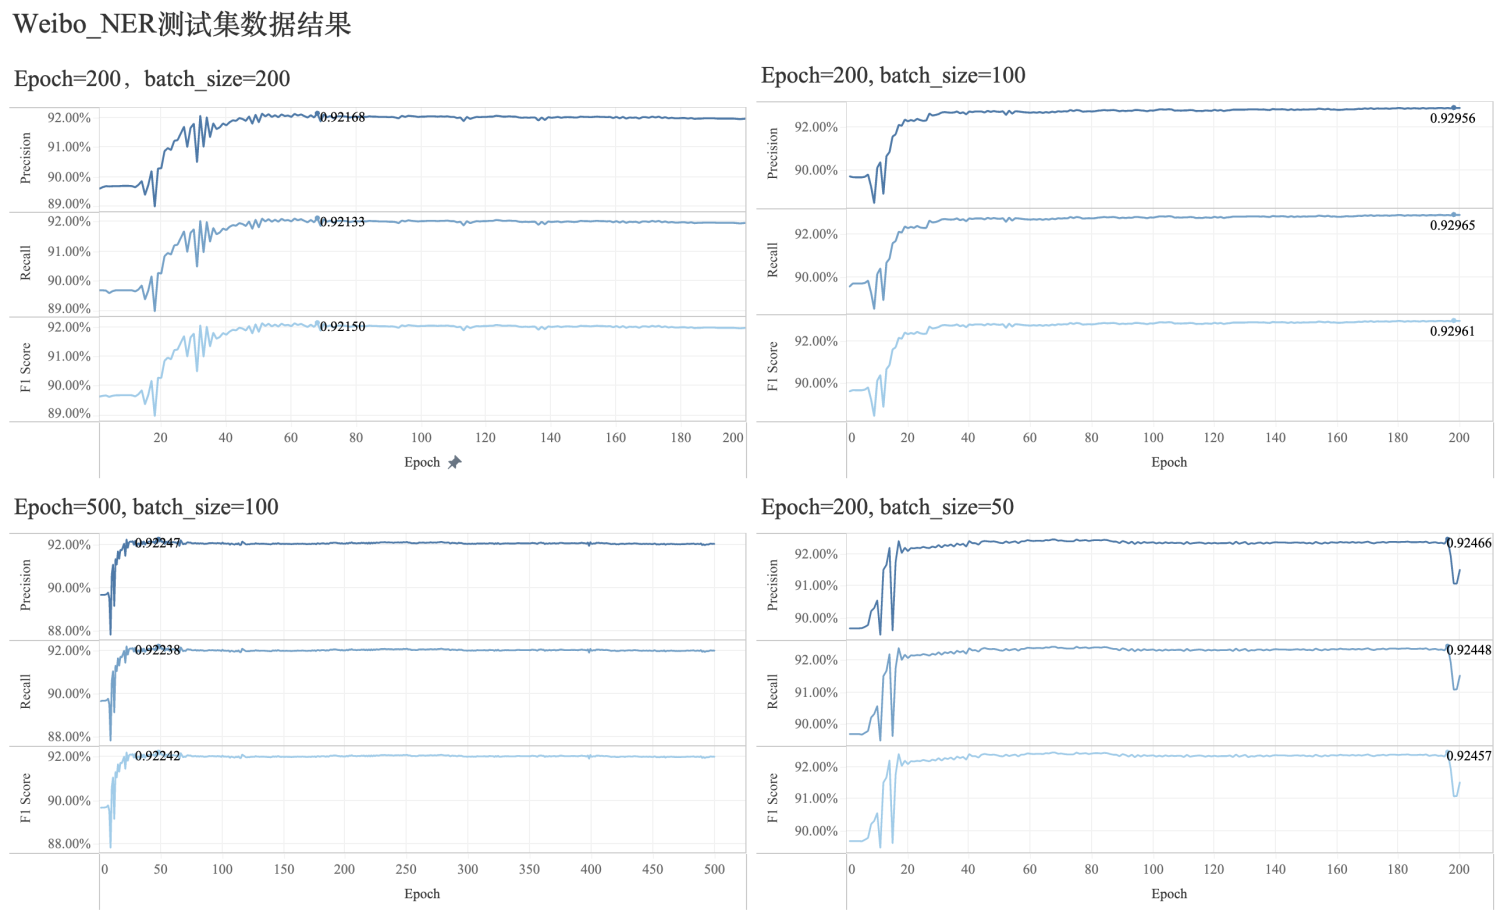
\includegraphics[width=14cm]{figures/weibo_ner_result.png}
    \caption{Weibo NER数据集测试结果}
\end{figure}

分别将epoch和batch\_size设置为(200, 200), (200, 100), (200, 50), (500, 100),Precision、Recall和F1 score随epoch变化
的趋势如图~\ref{fig:weibo_result}所示。可以看到Weibo数据集的字符级命名实体识别效果在(200, 100)的参数设置下F1值可以接近
93\%。


\subsubsection{MSRA数据集结果}

\begin{figure}[!htp]
    \centering
    \label{fig:MSRA_result}
    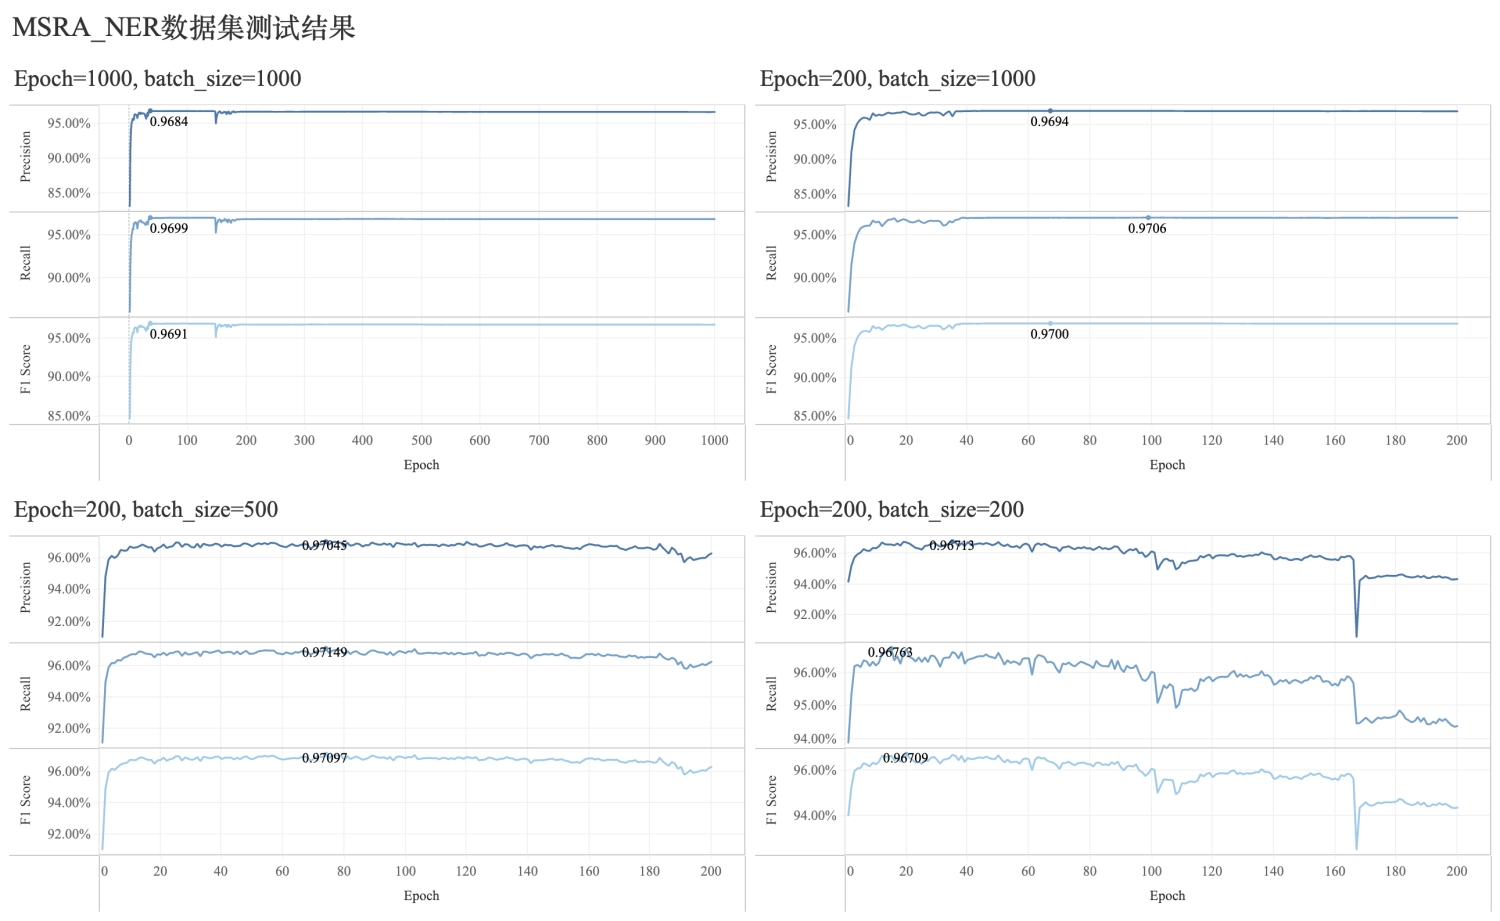
\includegraphics[width=14cm]{figures/MSRA_ner_result.png}
    \caption{MSRA数据集测试结果}
\end{figure}

分别将epoch和batch\_size设置为(1000, 1000)、(200, 1000)、(200, 500)、(200, 200),Precision、Recall和F1 score随epoch变化
的趋势如图~\ref{fig:MSRA_result}所示。可以看到MSRA数据集的字符级命名实体识别效果在(200, 500)的参数设置下F1值可以超过97\%。
